\documentclass{report}
\usepackage{graphicx}
\usepackage{framed}
\usepackage{verbatim}
\usepackage[section]{placeins}
\usepackage{titlesec}
\newcommand{\sectionbreak}{\clearpage}
\usepackage{hyperref}
\usepackage{circuitikz}
\usepackage{tikz}
\usepackage{pgfplots}
\usepackage[utf8]{inputenc}

\title{Laboratorijas darba № 1 atskaite 
   }
\author{Konstantins Glaskovs  }
\date{May 2018}

\begin{document}
\maketitle
%=====================================
\chapter{Teorētiskā daļa}
Uzdevums bija apēķinat spriegumus uz rezistoriem dotajā shēmā. Sprieguma avota V1 sprieguma
vērtību U (Voltos) izvēlieties daļskaitli, kas būtu Jūsu apliecības pēdējie trīs cipari dalīti ar
10. Mans apliecības numurs ir ‘171REB115’, tatād 115/10= 11.5, tad no tas sēkojam, kā V1 = 11.5 (Volti), R1 ir apliecības pēdējo 3 ciparu otrais
numurs+1, R2 ir apliecības numura pēdējais cipars +1.
Tātad ‘171REB115’, 115 ir pēdejie trīs cipari mana apliecības numura, lai noteikt ar ko ir vienāds R1,mūms vajag pie otra cipara (no skaitļa 115) pievienot 1. No tam sekojam 1+1=2, tad ‘R1=2’.Lai noteikt ar ko ir vienāds R2, mūms vajag pie treša cipara (no skaitļa 115) pivienot arī 1, ka iepriekšaja gadījuma. Tad, 5+1=6 ‘R2=6’. 
\begin{center}
\begin{circuitikz}[american voltages]
\draw
  (0,0.7) to [short] (5,0.7)
  to [V] (5,2) 
  to [R] (5,4) 
  to [short] (4,4) 
  (0,0.7) to [open] (0,0.7) 
  to [short] (0,4) 
  to [R] (4,4);
  \end{circuitikz}
  \end{center}
\begin{figure}
\begin{center}
\begin{tikzpicture}
\begin{axis}[
    xlabel=$R2$,
    ylabel=$U_{R2}$
    ]
\addplot[color=red,mark=*] coordinates {
		(5,8.21)
		(10,9.58)
		(15,10.1)
		(20,10.5)
		(25,10.6)
		(30,10.7)
		(40,10.8)
		(45,10.9)
		(50,11.2)
	};
\end{axis}
\end{tikzpicture}
\caption{$U_{R2}$=\textit{f}(\textit{R2}) grafiks, pēc sweep simulācijas datiem.}\label{graph:1}
\end{center}
\end{figure}

\section{Ķēdes aprēķins}

\begin {table}[h]
\begin{tabular}{c|c}
\hline
     $R1$ & 2 Om \\
     \hline
     $R2$ & 6Om \\
     \hline
     $V1$ & 11.5 V \\
     \hline
     $U_{R2}$ & 11.5 \\
     \hline
     $U_{R1}$ & 8.625 \\
     \hline
     
\end{tabular}
\caption {Sprieguma un pretestības tabula}
\end {table}
\begin{figure}[h]
    \centering
    \rotatebox{0}{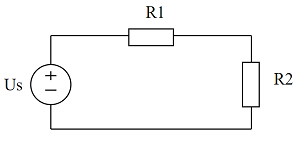
\includegraphics[scale=1, trim={12cm 5cm 10cm 10cm},clip]{12.png}}
    \caption{Shēma}
    \label{fig:my_label1}
\end{figure}

\chapter{Praktiskā daļa}
\section{Darbs ar GEDA programmām}
\subsection{darbs ar gschem}
        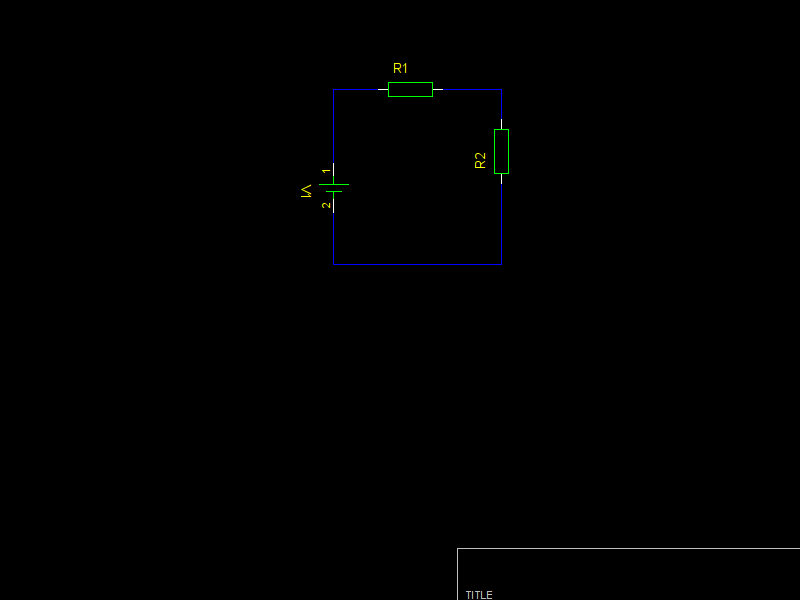
\includegraphics[width=12cm, height=6cm]{01.png}

            \caption{Figure 2.1.1: Elektriska shēma gschem vidē}
\subsection{darbs ar gnetlist}

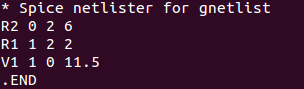
\includegraphics[width=5cm, height=3cm]{f.png}
\caption{Figure 2.1.2: Rezultātu parbaude ar gnetlist}

\subsection{darbs ar ngspice}
\begin{figure}[h]
        \centering
        \rotatebox{0}{{\frame{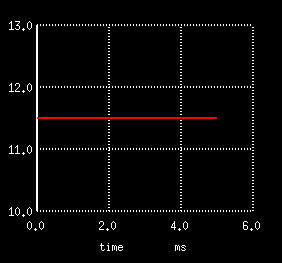
\includegraphics[scale=1]{c.png}}}}
        \label{fig:my_label2}
    \end{figure}
    \begin{figure}[h]
         \centering
        \rotatebox{0}{{\frame{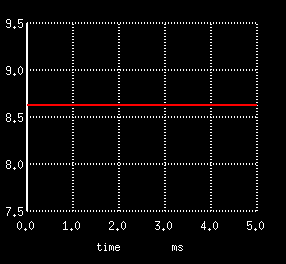
\includegraphics[scale=1]{z.png}}}}
        \caption{NGspice iegūtaie sprieguma grafiki}
        \label{fig:my_label3}
\end{figure}
\section{Darbs ar QUCS programmām}
\begin{figure}[h]
        \centering
        \rotatebox{0}{{\frame{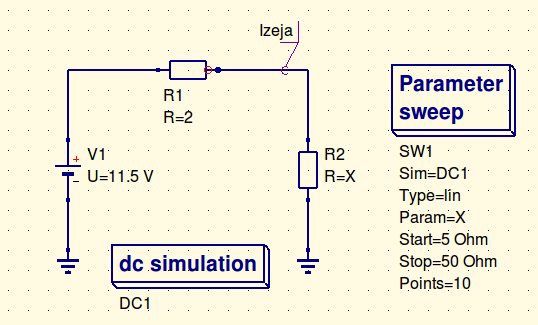
\includegraphics[scale=0.4, trim={25cm 10cm 35cm 21cm},clip]{a.png}}}}
        \caption{QUCS Shēmas modelis}
        \label{fig:my_label4}
    \end{figure}
    
    
    
    
    

    
    
    
    
    
    
    
    
    
    
    \subsection{Tabula un grafiks}
    \begin{figure}[h]
        \centering
        \rotatebox{0}{\frame{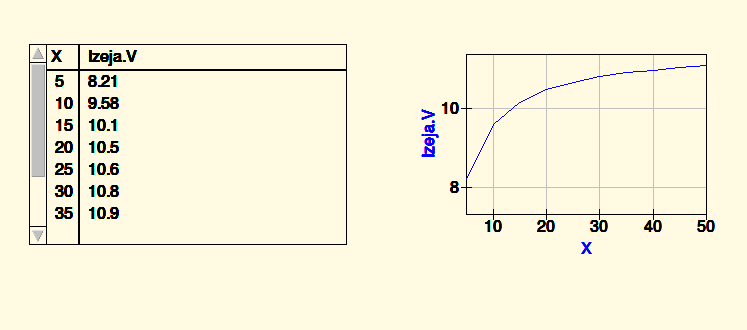
\includegraphics[scale=0.4, trim={25cm 15cm 35cm 35cm},clip]{b.png}}}
        \caption{Iegūtie rezultāti QUCS}
        \label{fig:my_label5}
\end{figure}
\begin{thebibliography}{9}
\bibitem{a_1}
Berga, I,. Ceske, E., Čekstere, I. u.c. 
\textit{Siguldas novadmācība}. (Latvia) 
[\textit{Siguldas novadmācība}]
Berga, I,. Ceske, E., Čekstere, I. u.c. Rīga: Preses nams, 2002. 186 lpp. ISBN 9984-19-250-4.

\bibitem{a_2} 
Joseph Heller
\textit{Catch-22}. 
Published September 4th 2004 by Simon and Schuster (first published 1961)
\end{thebibliography}

\end{document}


